\section{Uniform Laws of Large Numbers {(Ch.~4)}}
\subsection{Motivation}
\begin{definition}[Glivenko-Cantelli class]
We say $\mathcal{F}$ is Glivenko-Cantelli class if
$$ \norm{P_n - P}_{\mathcal{F}} := \sup_{f \in \mathcal{F}} \bigg| \frac{1}{n} \sum_{i=1}^n f(X_i) - \EE f(X_i) \bigg| \longrightarrow 0,
$$
in probability as $n \rightarrow 0$.
\end{definition}
\subsection{A uniform law via Rademacher complexity}
\begin{theorem}[Uniform law of large number] For $b$-uniformly bounded $\mathcal{F}$, we have
\begin{align*}
    P\left(\sup_{f\in \mathcal{F}} R(f) - R_n(f) \geq 2 \mathcal{R}_n(\mathcal{F}) + t\right) \leq e^{-\frac{nt^2}{2b^2}}.
\end{align*}
Here, population risk is $R(f) = \mathbb{E} f(x)$ and empirical risk is $R_n(f) = \frac{1}{n} \sum_{i=1}^n f(x_i)$. The Rademacher complexity is
\begin{align*}
    \mathcal{R}_{n}(\mathcal{F})=\mathbb{E}_{\epsilon} \sup _{h \in \mathcal{H}} \frac{1}{n} \sum_{i=1}^{n} \epsilon_{i} h(z_i), \quad \epsilon_i \sim \mathrm{Red}(\{-1, 1\})
\end{align*}
\end{theorem}
\begin{proof}
1. \textbf{Concentration around mean}. Let's denote
$$g_n(x_{1:n}) :=   \sup_{f \in \mathcal{F}} R(f) - R_n(f)= \sup_{f \in \mathcal{F}} \frac{1}{n} \sum_{i=1}^n f(x_i) - \EE{f(x)}.$$
Let $z = (x_1, \cdots, x_k, \cdots, x_n)$ and $z^{\backslash k} = (x_1, \cdots, x'_k, \cdots, x_n)$,
\begin{align*}
& \left|g_{n}(z)-g_{n}\left(z^{\backslash k}\right)\right| \\
= & \left|\sup _{h \in \mathcal{H}} \frac{1}{n} \sum_{i}\left[h\left(z_{i}\right)-\mathbb{E} h\right]-\sup _{\tilde{h} \in \mathcal{H}} \frac{1}{n} \sum_{i}\left[\tilde{h}\left(z_{i}^{\backslash k}\right)-\mathbb{E} \tilde{h}\right]\right| \\
\leq & \left|\sup _{h \in \mathcal{H}} \frac{\sum_{i} h\left(z_{i}\right)-h\left(z_{i}^{\backslash k}\right)}{n}\right| \leq\left|\sup _{h \in \mathcal{H}} \frac{h\left(x_{k}\right)-h\left(x_{k}^{\prime}\right)}{n}\right| \leq \frac{2 b}{n},
\end{align*}
which means $g_n$ has Lipschitz property.
Using McDiarmid inequality, $P\left(g_{n}(X) - \mathbb{E}g_{n}(X) \geq t\right) \leq e^{-\frac{n t^{2}}{2 b^{2}}}$.


2. \textbf{Upper bound on mean}. Using symmetrization technique and the definition of Rademacher complexity, we have
\begin{align*}
    \mathbb{E} g_n(X) & = \E{X}{\sup_{f \in \mathcal{F}} \frac{1}{n} \sum_{i=1}^n f(x_i) - \EE{f(x)}} \\
    & \leq \E{X, Y}{\sup_{f \in \mathcal{F}} \frac{1}{n} \sum_{i=1}^n f(x_i) - f(y_i)} & (\text{symmetrize}) \\
    & = \E{X, Y, \epsilon}{\sup_{f \in \mathcal{F}} \frac{1}{n} \sum_{i=1}^n \epsilon (f(x_i) - f(y_i))} & (\text{plug in } \epsilon) \\
    & \leq 2 \E{X, \epsilon}{\sup_{f \in \mathcal{F}} \frac{1}{n} \sum_{i=1}^n \epsilon f(x_i)} = 2 \mathcal{R}_n(\mathcal{F}).
\end{align*}
Combining these two parts, we have the desired theorem that $P\left(g_{n}(X) - 2\mathcal{R}_n(\mathcal{F}) \geq t\right) \leq e^{-\frac{n t^{2}}{2 b^{2}}}$.
\end{proof}

\begin{theorem}[Uniform law - corollary] If $\mathcal{R}_n(\mathcal{F}) = o(1)$, then when $n \rightarrow \infty$, we have
\begin{align*}
    \sup_{f\in \mathcal{F}} R(f) - R_n(f) \longrightarrow 0, \quad (a.s.)
\end{align*}
In other words, $\mathcal{R}_n(\mathcal{F}) = o(1)$ implies that $\mathcal{F}$ is a Glivenko-Cantelli class.
\end{theorem}
\begin{proof}
Let $\mathcal{E}_n(\alpha)$ denote the event that $\sup_{f\in \mathcal{F}} R(f) - R_n(f) \geq \alpha$. The uniform law shows that
\begin{align*}
    P\left(\mathcal{E}_n( 2\mathcal{R}_n(\mathcal{H}) + t )\right) & \leq  e^{-\frac{nt^2}{2b^2}}.
\end{align*}
Using union bound,  $\forall t > 0$, we have,
\begin{align*}
   \sum_{n=1}^{\infty} P(\mathcal{E}_n(2t)) & \leq \sum_{n=1}^{k} P\left(\mathcal{E}_n\left(2t\right)\right)  + \sum_{n=k+1}^\infty P\left(\mathcal{E}_n\left(2\mathcal{R}_n(\mathcal{H}) + t \right)\right) \\
    & \leq \sum_{n=1}^{k} P\left(\mathcal{E}_n\left(2t\right)\right) + \sum_{n=k+1}^\infty  e^{-\frac{nt^2}{2b^2}} < \infty.
\end{align*}
The $k$ is chosen such that when $n > k$, $\mathcal{R}_n(f) < \frac{t}{2}$. Such $k$ must exist, since $\mathcal{R}_n(f) = o(1)$.
Using the Borel-Cantalli lemma, we show that
\begin{align*}
    P\left(\lim_{n \rightarrow \infty} \sup \mathcal{E}_n(2t) \right) = 0.
\end{align*}
Considering that $t$ can be arbitrarily small, we have
\begin{align*}
    P\left(\lim_{n \rightarrow \infty} \sup_{f\in \mathcal{F}} R(f) - R_n(f) = 0 \right) = 1.
\end{align*}
\end{proof}

\subsection{Upper bounds on the Rademacher complexity}
\begin{definition}[Growth function]
The growth function $N_\mathcal{H}$ for a hypothesis space $\mathcal{H}$ is defined as: $\forall m \in \mathbb{N}$,
\begin{align*}
    N_{\mathcal{H}}(n) := \sup_{z_{1:n} \subseteq Z }\left|\left\{\left(h\left(z_{1}\right), \cdots, h\left(z_{n}\right)\right) \mid h \in \mathcal{H}\right\}\right|
\end{align*}
\end{definition}
\textbf{Remark}: Growth function measures the maximum number of distinct ways in which m points can be classified using hypotheses in $\mathcal{H}$.

\begin{theorem}[Massart lemma]
For a data set $z_{1:n} = \{z_1, \cdots, z_n\}$, the hypothesis $h: Z \rightarrow\{0,1\}$ and the hypothesis space $\mathcal{H}(z_{1:n}):=\{(h(z_1), \cdots, h(z_n)) \mid h \in \mathcal{H}\}$, we have
\begin{align*}
    {\mathcal{R}}_{n}\left(\mathcal{H}\right):=\mathbb{E}_{\epsilon}\left[ \sup _{h \in \mathcal{H}} \frac{1}{n} \sum_{i=1}^{n} \epsilon_{i} h\left(z_{i}\right)\right] \leq 2 \sqrt{\frac{\log \left|\mathcal{H}\left(z_{1:n}\right)\right|}{n}}
\end{align*}
\end{theorem}
\textbf{Remark}: Using this result, we can now bound the Rademacher complexity in terms of the growth function.

\vspace{1em}
\begin{proof}
First, we show that $\epsilon^T \theta$ is $\sqrt{n}$ sub-Gaussian. Using the independence of $z$, $\forall \lambda \in \mathbb{R}$, we have
\begin{align*}
\mathbb{E}_\epsilon \left[ \exp(\lambda \epsilon^\top\theta)\right] & = \mathbb{E}_\epsilon \left[\exp \left( \lambda \sum_{i=1}^n \epsilon_i \theta_i \right) \right] \\
& = \mathbb{E}_{\epsilon_1} \left[\exp \left(\lambda\epsilon_1 \theta_1 \right) \right] \cdots \mathbb{E}_{\epsilon_n} \left[\exp \left(\lambda \epsilon_n \theta_n \right) \right]\\
& \leq \exp\left(\frac{\lambda^2 \theta_1^2}{2} + \cdots + \frac{\lambda^2 \theta_n^2}{2} \right) \leq \exp\left(\frac{\lambda^2 n}{2}\right).
\end{align*}
Next, using the Gaussian maxima, we get
\begin{align*}
    \mathbb{E} \max _{\theta \in \mathbb{T}} \epsilon^T \theta \leq 2 \sqrt{n \log \left|\mathcal{H}\left(z_{1}^{n}\right)\right|}
\end{align*}
Then, we can get the intended results.
\end{proof}

\begin{definition}[VC Dimension]
The VC dimension of $\mathcal{H}$ is  the biggest $n \in \mathbb{N}$ such that there exists $n$ samples in $\mathcal{H}$ which can be arbitrarily scattered by a binary classifier, i.e.,
\begin{align*}
    d_{VC} = \max_{n \in \mathbb{N}} n, \quad \text{s.t. } \exists z_{1:n} \in Z^n, \mathcal{H}(z_{1:n}) = \{0,1\}^n.
\end{align*}
Here, $\mathcal{H}(z_{1:n}):=\{(h(z_1), \cdots, h(z_n)) \mid h \in \mathcal{H}\}$。
\end{definition}
\textbf{Remark}: Finite VC dimension can make $\mathcal{H}$ a Glivenko-Cantelli class.

\begin{theorem}[Sauer-Shelah]
For a space $\mathcal{H}$ with VC dimension $d_{VC}$, for any $z_1, \cdots, z_n$, we have growth function
\begin{align*}
    N_\mathcal{H}(n) := \sup_{z_{1:n} \in Z^n} |\mathcal{H}(z_{1:n})| \leq (n + 1)^{d_{VC}}, \quad \forall n \geq d_{VC}
\end{align*}
\end{theorem}
\begin{proof}
Proof by combination algebra. See the Chapter 4.3 for more details.
\end{proof}

\begin{theorem}[Rademacher contraction]
For any $\mathbb{T} \subseteq \R^n$ and $\ell : \R^n \rightarrow \R^n$ with univariate $L$-Lipschitz
functions it holds that
\begin{align*}
    \tilde{\mathcal{R}}_{n}(\ell \circ \mathbb{T}) \leq L \tilde{\mathcal{R}}_{n}(\mathbb{T})
\end{align*}
\end{theorem}
\begin{proof}
See the slides of Lecture 5.
\end{proof}



\section{Non-uniform Learnability (Lec. 6-7)}

\subsection{Structural risk minimization (SRM)}
\begin{definition}[SRM]
Say we have a nested family of function spaces $\mathcal{H}_{1} \subset \mathcal{H}_{2} \subset \cdots$, where $\mathcal{H} = \bigcup_k \mathcal{H}_{k} $. For each $\mathcal{H}_k$ define the event
$$
E_{k, h}=\left\{R(h)-R_{n}(h) \leq c \sqrt{\frac{\log \left(1 / \delta_{k}\right)}{n}}+2 \mathcal{R}_{n}\left(\mathcal{H}_{k}\right)\right\}.
$$
\end{definition}

\begin{theorem}[Uniform law via the SRM]
Define $k(h) = \min \{k \mid f \in \mathcal{H}_k\}$ which for each $h$ finds the minimum set $\mathcal{H}_k$.

If $P(\bigcap_{h \in \mathcal{H}_k} E_{k, h} ) \geq 1 - \delta_k$ for each $k$ and if $\sum_k \delta_k \leq \delta$, with probability at least $1 - \delta$,
$$
\sup _{h \in \mathcal{H}} R(h)-R_{n}(h) \leq c \sqrt{\frac{\log \left(1 / \delta_{k(h)}\right)}{n}}+2 \mathcal{R}_{n}\left(\mathcal{H}_{k(h)}\right)
$$
\end{theorem}
\begin{proof}
Observe that
\begin{align*}
A := & \left\{\sup _{h \in \mathcal{H}} R(h)-R_{n}(h) \leq c \sqrt{\frac{\log \left(1 / \delta_{k(h)}\right)}{n}}+2 \mathcal{R}_{n}\left(\mathcal{H}_{k(h)}\right)\right\} \\
=& \cap_{h \in \mathcal{H}} \cap_{k: h \in \mathcal{H}_{k}} E_{k, h}=\cap_{k \in \mathbb{N}} \cap_{h \in \mathcal{H}_{k}} E_{k, h}
\end{align*}
Then, we can use the union bound,
\begin{align*}
    P(A)=1-P\left(\cup_{k \in \mathbb{N}} \cup_{h \in \mathcal{H}_{k}} E_{k, h}\right) \geq 1-\sum_{k} \delta_{k} \geq 1-\delta,
\end{align*}
which concludes the proof.
\end{proof}
\begin{center}
    \tikzset{every picture/.style={line width=0.75pt}} %set default line width to 0.75pt        

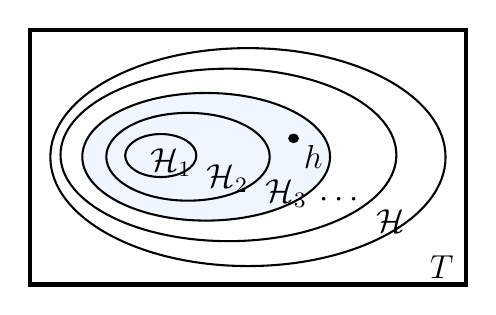
\begin{tikzpicture}[x=0.75pt,y=0.75pt,yscale=-0.6,xscale=0.7]
%uncomment if require: \path (0,365); %set diagram left start at 0, and has height of 365

%Shape: Circle [id:dp5556054645273254] 
\draw  [fill={rgb, 255:red, 0; green, 0; blue, 0 }  ,fill opacity=1 ] (376.28,140.87) .. controls (376.28,139.24) and (377.6,137.91) .. (379.24,137.91) .. controls (380.87,137.91) and (382.19,139.24) .. (382.19,140.87) .. controls (382.19,142.5) and (380.87,143.83) .. (379.24,143.83) .. controls (377.6,143.83) and (376.28,142.5) .. (376.28,140.87) -- cycle ;
%Shape: Rectangle [id:dp5281419369218745] 
\draw  [line width=1.5]  (197.67,47.75) -- (498,47.75) -- (498,252.25) -- (197.67,252.25) -- cycle ;
%Shape: Ellipse [id:dp5525274261812825] 
\draw   (218.84,148.25) .. controls (218.84,110) and (270.58,79) .. (334.42,79) .. controls (398.25,79) and (450,110) .. (450,148.25) .. controls (450,186.49) and (398.25,217.5) .. (334.42,217.5) .. controls (270.58,217.5) and (218.84,186.49) .. (218.84,148.25) -- cycle ;
%Shape: Ellipse [id:dp47565683667848213] 
\draw  [fill={rgb, 255:red, 239; green, 246; blue, 255 }  ,fill opacity=1 ] (233.84,149.75) .. controls (233.84,121.44) and (272,98.5) .. (319.09,98.5) .. controls (366.17,98.5) and (404.34,121.44) .. (404.34,149.75) .. controls (404.34,178.05) and (366.17,201) .. (319.09,201) .. controls (272,201) and (233.84,178.05) .. (233.84,149.75) -- cycle ;
%Shape: Ellipse [id:dp8225386024812087] 
\draw   (250.34,149.75) .. controls (250.34,130.28) and (275.52,114.5) .. (306.59,114.5) .. controls (337.65,114.5) and (362.84,130.28) .. (362.84,149.75) .. controls (362.84,169.22) and (337.65,185) .. (306.59,185) .. controls (275.52,185) and (250.34,169.22) .. (250.34,149.75) -- cycle ;
%Shape: Ellipse [id:dp012503998897681612] 
\draw   (263.34,148.75) .. controls (263.34,139.22) and (274.3,131.5) .. (287.84,131.5) .. controls (301.37,131.5) and (312.34,139.22) .. (312.34,148.75) .. controls (312.34,158.27) and (301.37,166) .. (287.84,166) .. controls (274.3,166) and (263.34,158.27) .. (263.34,148.75) -- cycle ;
%Shape: Ellipse [id:dp7411816000021694] 
\draw   (211.84,150) .. controls (211.84,101.67) and (272.72,62.5) .. (347.84,62.5) .. controls (422.95,62.5) and (483.84,101.67) .. (483.84,150) .. controls (483.84,198.32) and (422.95,237.5) .. (347.84,237.5) .. controls (272.72,237.5) and (211.84,198.32) .. (211.84,150) -- cycle ;
%Shape: Circle [id:dp06594432447625231] 
\draw  [fill={rgb, 255:red, 0; green, 0; blue, 0 }  ,fill opacity=1 ] (376.28,134.96) .. controls (376.28,133.33) and (377.6,132) .. (379.24,132) .. controls (380.87,132) and (382.19,133.33) .. (382.19,134.96) .. controls (382.19,136.59) and (380.87,137.91) .. (379.24,137.91) .. controls (377.6,137.91) and (376.28,136.59) .. (376.28,134.96) -- cycle ;

% Text Node
\draw (471,226.4) node [anchor=north west][inner sep=0.75pt]    {\large$T$};
% Text Node
\draw (278.5,140.9) node [anchor=north west][inner sep=0.75pt]    {\large $\mathcal{H}_{1}$};
% Text Node
\draw (317.5,153.4) node [anchor=north west][inner sep=0.75pt]    {\large$\mathcal{H}_{2}$};
% Text Node
\draw (358,165.9) node [anchor=north west][inner sep=0.75pt]    {\large$\mathcal{H}_{3}$};
% Text Node
\draw (395,176.4) node [anchor=north west][inner sep=0.75pt]    {\large$\cdots $};
% Text Node
\draw (434,189.9) node [anchor=north west][inner sep=0.75pt]    {\large$\mathcal{H}$};
% Text Node
\draw (384.19,138.36) node [anchor=north west][inner sep=0.75pt]    {\large$h$};
\end{tikzpicture}

\caption{\textbf{Figure}: Demonstration of SRM when $k(h)=3$.}
\end{center}
\subsection{Margin bound for linear classifiers}
\begin{definition}[Linear classifiers]
Define the empirical risk
$$
R_{n}^{\gamma}(f)=\frac{1}{n} \sum_{i=1}^{n} \mathbbm{1}_{y_{i} f\left(x_{i}\right) \leq \gamma},
$$
and the population risk
$$
R^{\gamma}(f) := \EE_{X, Y}  \mathbbm{1}_{y_{i} f\left(x_{i}\right) \leq \gamma}.
$$
\end{definition}

\begin{theorem}[Rademacher complexity of $L_2$-bounded linear class]
For a class of linear functions $\mathcal{F}_{B, 2}=\left\{f(x)=\langle w, x\rangle:\|w\|_{2} \leq B\right\}$, we have
$$
{\mathcal{R}}_{n}\left(\mathcal{F}_{B, 2}
\right) \leq \frac{B \max _{i}\left\|x_{i}\right\|_{2}}{\sqrt{n}}
$$
\end{theorem}
\begin{proof}
Using the definition of Rademacher complexity and Cauchy's inequality, we have
\begin{align*}
n \cdot \mathcal{R}_n\left(\mathcal{F}_{B, 2}\right) &={\mathbb{E}}_\sigma\sup _{f \in \mathcal{F}_{B, 2}} \sum_{i=1}^{n} \sigma_{i} f(x_i)\\
&={\mathbb{E}_\sigma}\sup _{\|{w}\|_2 \leq B} \sum_{i=1}^{n} \sigma_{i}\left\langle{w}, x_{i}\right\rangle \\
&={\mathbb{E}_\sigma}\sup _{\|{w}\|_2 \leq B}\left\langle{w}, \sum_{i=1}^{n} \sigma_{i} x_{i}\right\rangle \\
& \leq B {\mathbb{E}_\sigma}\sqrt{\left\|\sum_{i=1}^{n} \sigma_{i} x_{i}\right\|^2_{2}} & (\text{Cauchy's}) \\
& \leq B \sqrt{\mathbb{E}_\sigma \left\|\sum_{i=1}^{n} \sigma_{i} x_{i}\right\|^2_{2}} & (\text{Jensen's})
\end{align*}
Finally, since the Rademacher variables $\sigma$ are independent, we have
\begin{align*}
{\mathbb{E}_\sigma}\left\|\sum_{i=1}^{m} \sigma_{i} x_{i}\right\|_{2}^{2}&={\mathbb{E}_\sigma}\sum_{i, j} \sigma_{i} \sigma_{j}\left\langle x_{i}, x_{j}\right\rangle\\
&=\sum_{i \neq j}\left\langle x_{i}, x_{j}\right\rangle \mathbb{E}_\sigma\left[\sigma_{i} \sigma_{j}\right]+\sum_{i=1}^{m}\left\langle x_{i}, x_{i}\right\rangle {\mathbb{E}_\sigma}[\sigma_{i}^{2}] \\
&=\sum_{i=1}^{m}\left\|x_{i}\right\|_{2}^{2} \leq n \max _{i}\left\|{x}_{i}\right\|_{2}^{2}.
\end{align*}
Plug into the previous inequality and we get the result.
\end{proof}

\begin{theorem}[Non-uniform margin bound \label{thm:non_uniform}]
If the assumptions are valid for any fixed $\gamma$, with probability at least $1 - \delta$, for any $f \in \mathcal{F}_{B}$, we have
$$
R^{0}(f)=P(y \neq \operatorname{sign}(f(x))) \leq R_{n}^{\gamma}(f)+\frac{2 D B}{\gamma \sqrt{n}}+c \sqrt{\frac{\log (1 / \delta)}{n}}
$$
\end{theorem}
\begin{proof}
Please refer to Lec. 7 and Exercise class 1.
\end{proof}

\subsection{Margin bounds for SVM}

\begin{theorem}[Non-uniform margin bound for SVM\label{thm:svm}]
If the assumptions are valid for any fixed $\gamma$, with probability at least $1 - \delta$, for any $f \in \mathcal{F}_{B}$, we have
$$
P(y \neq \operatorname{sign}(f(x))) \leq R_{n}^{\gamma}(f)+\frac{2 D \norm{w^*}_2}{ \sqrt{n}}+c \sqrt{\frac{\log (1 / \delta)}{n}}
$$
\end{theorem}
\begin{proof}
Using the margin bound theorem (Thm.~\ref{thm:non_uniform}) with $\gamma = 1$ then yields the result.
\end{proof}

\begin{theorem}[Uniform margin bound for SVM]
\begin{align*}
\mathbb{P}(y f_{SVM}(x)<0) \leq & \frac{2 e D\left\|w_{S V M}\right\|_{2}}{\sqrt{n}} \\ & +c \sqrt{\frac{\log (1 / \delta)+\log \left(4 \log \left\|w_{S V M}\right\|_{2}\right)}{n}}
\end{align*}
\end{theorem}
\begin{proof}
Choose $B_k = e^k$ and the nested function space is $\mathcal{F}_{B_k} := \{ w \mid \norm{w} \leq B_k \}$. According to the Non-uniform margin bound for SVM (Thm.~\ref{thm:svm}), let $\delta_k = \frac{\delta}{2k^2}$.
Then $k(w) = \ceil{\log \norm{w}}$ and thus $B_{k(w)} = \norm{w} e$ and 
$$
\frac{1}{\delta_{k(w)}}=\frac{2 (k(w))^{2}}{\delta} \leq \frac{2(2 \log \|w\|)^{2}}{\delta}.
$$
Plugging in the quantities yields the results with probability at
\begin{align*}
    1 - \sum_{i=1}^\infty \delta_k = 1 - \delta \sum_{i=1}^\infty \frac{1}{2k^2} \geq 1 - \delta,
\end{align*}
which concludes the proof.
\end{proof}